\documentclass[border=10pt]{standalone}
\usepackage{tikz}
\usetikzlibrary{calc}

\begin{document}
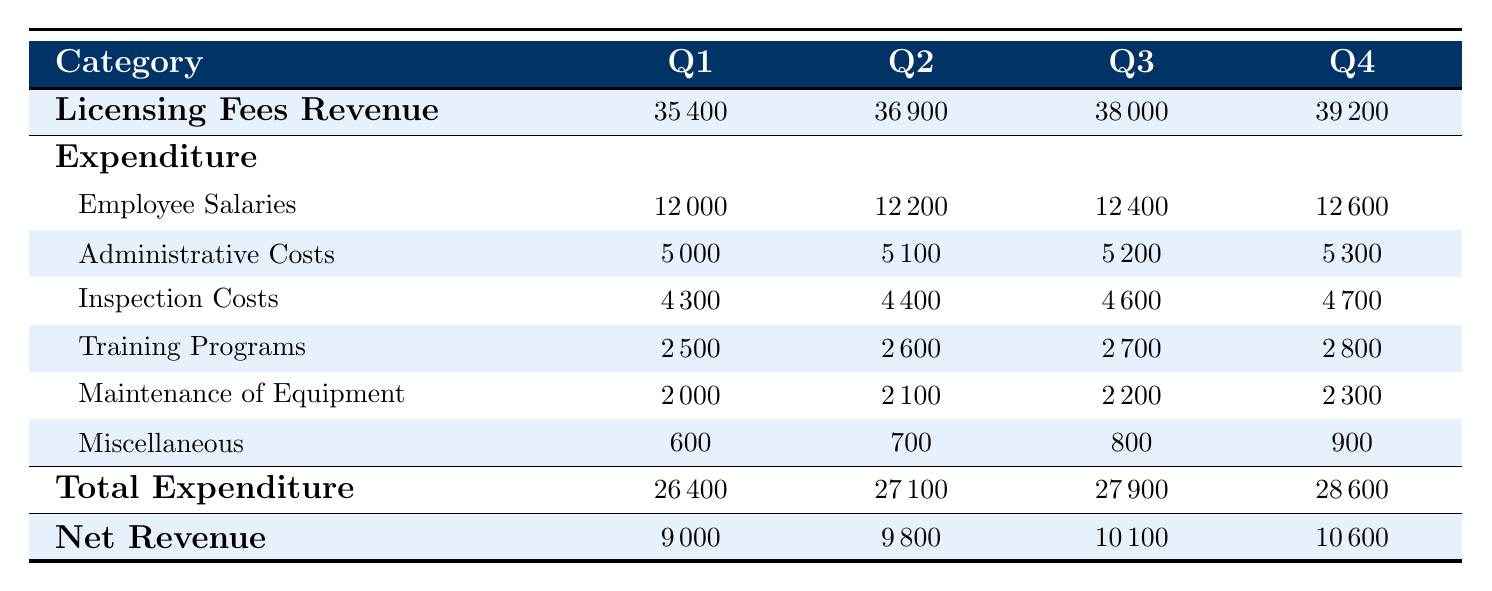
\begin{tikzpicture}[x=1cm,y=0.6cm]
  % Basic dimensions
  \def\catwidth{7}
  \def\colwidth{2.8}
  \def\ncols{5} % category + 4 quarters
  \def\tablewidth{\catwidth+4*\colwidth}
  % Row y-positions (from top = 0, going downward)
  % r0 header
  % r1 revenue
  % r2 Expenditure label
  % r3-8 expenditure detail lines
  % r9 Total Expenditure
  % r10 Net Revenue
  \foreach \i[count=\j] in {0,...,10} {
    \coordinate (row\i) at (0,-\i);
  }
  
  % Colors
  \definecolor{darkblue}{RGB}{0,51,102}
  \definecolor{lightblue}{RGB}{230,241,252}
  
  % Booktabs-style top and bottom rules
  \draw[very thick] (0,0.25) -- (\tablewidth,0.25);
  \draw[very thick] (0,-11) -- (\tablewidth,-11);
  
  % Column x positions
  \coordinate (c0) at (0,0);
  \coordinate (c1) at (\catwidth,0);
  \coordinate (c2) at (\catwidth+\colwidth,0);
  \coordinate (c3) at (\catwidth+2*\colwidth,0);
  \coordinate (c4) at (\catwidth+3*\colwidth,0);
  \coordinate (c5) at (\tablewidth,0);
  
  % Header background
  \fill[darkblue] (0,0) rectangle (\tablewidth,-1);
  
  % Header bottom line
  \draw[very thick] (0,-1) -- (\tablewidth,-1);
  
  % Header text
  \node[white,font=\bfseries\large,anchor=west] at (0.2,-0.5) {Category};
  \node[white,font=\bfseries\large] at ($(c1)!0.5!(c2)+(0,-0.5)$) {Q1};
  \node[white,font=\bfseries\large] at ($(c2)!0.5!(c3)+(0,-0.5)$) {Q2};
  \node[white,font=\bfseries\large] at ($(c3)!0.5!(c4)+(0,-0.5)$) {Q3};
  \node[white,font=\bfseries\large] at ($(c4)!0.5!(c5)+(0,-0.5)$) {Q4};
  
  % Shaded rows (revenue row, alternating expenditure rows, Net Revenue)
  \fill[lightblue] (0,-1) rectangle (\tablewidth,-2);  % Licensing Fees Revenue
  \fill[lightblue] (0,-4) rectangle (\tablewidth,-5);  % Administrative Costs
  \fill[lightblue] (0,-6) rectangle (\tablewidth,-7);  % Training Programs
  \fill[lightblue] (0,-8) rectangle (\tablewidth,-9);  % Miscellaneous
  \fill[lightblue] (0,-10) rectangle (\tablewidth,-11); % Net Revenue
  
  % Booktabs-style horizontal rules
  \draw[very thick] (0,-1) -- (\tablewidth,-1);  % below header
  \draw (0,-2) -- (\tablewidth,-2);             % below revenue
  \draw (0,-9) -- (\tablewidth,-9);             % above Total Expenditure
  \draw (0,-10) -- (\tablewidth,-10);           % above Net Revenue
  \draw[very thick] (0,-11) -- (\tablewidth,-11);% bottom rule
  
  % Text styles
  \tikzset{
    labelmain/.style={font=\bfseries\large,anchor=west},
    labelsub/.style={font=\normalsize,anchor=west},
    num/.style={font=\normalsize,anchor=center,xshift=-1.2cm}
  }
  
  % Row 1: Licensing Fees Revenue
  \node[labelmain] at (0.2,-1.5) {Licensing Fees Revenue};
  \node[num] at (\catwidth+\colwidth-0.2,-1.5) {35\,400};
  \node[num] at (\catwidth+2*\colwidth-0.2,-1.5) {36\,900};
  \node[num] at (\catwidth+3*\colwidth-0.2,-1.5) {38\,000};
  \node[num] at (\catwidth+4*\colwidth-0.2,-1.5) {39\,200};
  
  % Row 2: Expenditure headline
  \node[labelmain] at (0.2,-2.5) {Expenditure};
  
  % Expenditure subrows labels (indented)
  \def\indent{0.5}
  \node[labelsub] at (\indent,-3.5) {Employee Salaries};
  \node[labelsub] at (\indent,-4.5) {Administrative Costs};
  \node[labelsub] at (\indent,-5.5) {Inspection Costs};
  \node[labelsub] at (\indent,-6.5) {Training Programs};
  \node[labelsub] at (\indent,-7.5) {Maintenance of Equipment};
  \node[labelsub] at (\indent,-8.5) {Miscellaneous};
  
  % Expenditure numbers
  % Employee Salaries
  \node[num] at (\catwidth+\colwidth-0.2,-3.5) {12\,000};
  \node[num] at (\catwidth+2*\colwidth-0.2,-3.5) {12\,200};
  \node[num] at (\catwidth+3*\colwidth-0.2,-3.5) {12\,400};
  \node[num] at (\catwidth+4*\colwidth-0.2,-3.5) {12\,600};
  % Administrative Costs
  \node[num] at (\catwidth+\colwidth-0.2,-4.5) {5\,000};
  \node[num] at (\catwidth+2*\colwidth-0.2,-4.5) {5\,100};
  \node[num] at (\catwidth+3*\colwidth-0.2,-4.5) {5\,200};
  \node[num] at (\catwidth+4*\colwidth-0.2,-4.5) {5\,300};
  % Inspection Costs
  \node[num] at (\catwidth+\colwidth-0.2,-5.5) {4\,300};
  \node[num] at (\catwidth+2*\colwidth-0.2,-5.5) {4\,400};
  \node[num] at (\catwidth+3*\colwidth-0.2,-5.5) {4\,600};
  \node[num] at (\catwidth+4*\colwidth-0.2,-5.5) {4\,700};
  % Training Programs
  \node[num] at (\catwidth+\colwidth-0.2,-6.5) {2\,500};
  \node[num] at (\catwidth+2*\colwidth-0.2,-6.5) {2\,600};
  \node[num] at (\catwidth+3*\colwidth-0.2,-6.5) {2\,700};
  \node[num] at (\catwidth+4*\colwidth-0.2,-6.5) {2\,800};
  % Maintenance of Equipment
  \node[num] at (\catwidth+\colwidth-0.2,-7.5) {2\,000};
  \node[num] at (\catwidth+2*\colwidth-0.2,-7.5) {2\,100};
  \node[num] at (\catwidth+3*\colwidth-0.2,-7.5) {2\,200};
  \node[num] at (\catwidth+4*\colwidth-0.2,-7.5) {2\,300};
  % Miscellaneous
  \node[num] at (\catwidth+\colwidth-0.2,-8.5) {600};
  \node[num] at (\catwidth+2*\colwidth-0.2,-8.5) {700};
  \node[num] at (\catwidth+3*\colwidth-0.2,-8.5) {800};
  \node[num] at (\catwidth+4*\colwidth-0.2,-8.5) {900};
  
  % Total Expenditure row
  \node[labelmain] at (0.2,-9.5) {Total Expenditure};
  \node[num] at (\catwidth+\colwidth-0.2,-9.5) {26\,400};
  \node[num] at (\catwidth+2*\colwidth-0.2,-9.5) {27\,100};
  \node[num] at (\catwidth+3*\colwidth-0.2,-9.5) {27\,900};
  \node[num] at (\catwidth+4*\colwidth-0.2,-9.5) {28\,600};
  
  % Net Revenue row
  \node[labelmain] at (0.2,-10.5) {Net Revenue};
  \node[num] at (\catwidth+\colwidth-0.2,-10.5) {9\,000};
  \node[num] at (\catwidth+2*\colwidth-0.2,-10.5) {9\,800};
  \node[num] at (\catwidth+3*\colwidth-0.2,-10.5) {10\,100};
  \node[num] at (\catwidth+4*\colwidth-0.2,-10.5) {10\,600};
  
\end{tikzpicture}
\end{document}
